% 第5章
\section{実装}
  \label{sec:実装}
    \par 本章では,本研究で提案するCtoCシェアサイクルサービスの具体的な実装について述べる.システム全体は,大きく分けてスマートロックのプロトタイプ実装,数理最適化モデルの実装,そしてそれらを統合するAPIの開発の3つの要素から構成される.それぞれの要素について,詳細な実装手法を以下の節で説明する.
    \par まず,\ref{sec:スマートロックプロトタイプ実装}節にて,自転車の鍵をスマートロック化するためのプロトタイプ実装について解説し,次に,\ref{sec:数理最適化モデルの実装}節にて,\ref{sec:数理最適化ベースのマッチングモデルの設計}節で定式化した数理最適化モデルを実際のシステムに組み込む手法について説明する.最後に,\ref{sec:API開発}節にて,スマートロックと数理最適化モデルを統合し,外部からアクセス可能なサービスとするためのAPI開発について説明する.
  
  \subsection{スマートロックプロトタイプ実装}
    \label{sec:スマートロックプロトタイプ実装}
      \par \ref{sec:ハードウェア設計}項にて述べた通り,本研究ではハードウェアに関しては深入りせず,最終的な動作の確認のためのプロトタイプとして位置付けている.これは,ハードウェア開発に多くの時間とリソースを費やすのではなく,ソフトウェアシステム全体の動作に重点を置くためである.また,ハードウェアとソフトウェアのそれぞれについて切り分けて実装し,、個別に検証・改良を行いやすくする.ハードウェアでは,自転車の鍵をスマートロックとして解錠・施錠の最低限の動作の確認ができるベースを構築する.ソフトウェアにおいては2種類の認証手法を実装し,それぞれ解錠・施錠の処理が実行できるよう構築する.全体として,将来的に他の認証手法や追加機能を容易に統合できる柔軟なプラットフォームを提供することを目的とし,極力拡張性を持たせた自転車の鍵におけるスマートロックのプロトタイプとなるよう構築する.
      \par ハードウェアについては,一般的な自転車に標準装備されているシリンダー式のリング錠をベースとして,ESP32マイコンやサーボモーターを組み込み,スマートロックを構築する.NFCによる認証と指紋による認証はそれぞれ構築したスマートロックの右上にNFCタグや指紋認証センサーを組み込み,解錠するためのトリガーとする.ハードウェア全体としてのプロトタイプは図\ref{fig:スマートロックのハードウェア全体像}のようになる.図\ref{fig:スマートロックのハードウェア全体像}では認証手法にNFCを用いた場合の様子であるため,スマートロックの右上にNFCタグを組み込んでいるが,認証手法に指紋認証を用いる場合は図\ref{fig:スマートロックのハードウェア全体像}でNFCタグが組み込まれている部分を指紋認証センサに置き換えれば良い.
      \par この自転車のスマートキーを解錠させる仕組みとしては,マイコンで制御されたサーボモーターの回転数によって物理的に鍵を回転させる手順となる.この際にサーボモーターのトルクを無駄なく鍵の回転に利用するため,1立方センチメートル程度の大きさの木材を支柱として鍵に対して対角線上に取り付ける.このようにすることでサーボモーターの回転を間接的に利用することができる.
      \par ソフトウェアについては,NFCによる認証と指紋による認証で異なるため,それぞれについて言及する.
      \par まず,NFC認証の場合のソフトウェアの実装については,3つの外部アプリケーションを利用して構築する.
      
      \begin{figure}[b!]
        \centering
        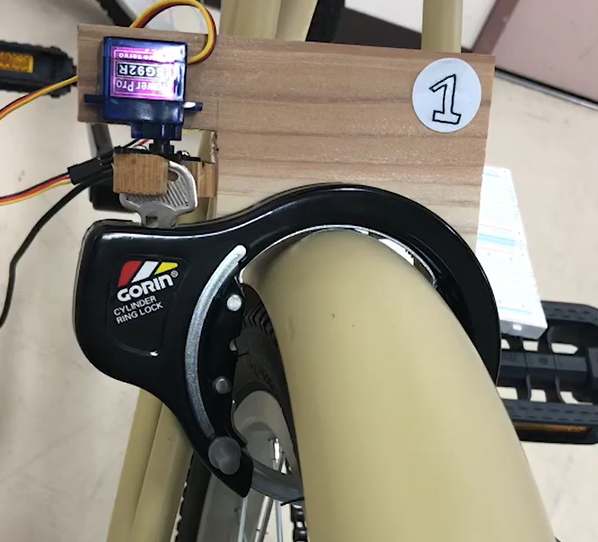
\includegraphics[scale=0.5]
        {figures/smartlock_hardware.png}
        \caption{スマートロックのハードウェア全体像}
        \label{fig:スマートロックのハードウェア全体像}
      \end{figure}
      
      \par 1つ目は,WebアプリケーションやAndroid/iOSアプリケーションを用いて電子機器を遠隔操作することができるIoTプラットフォーム「Blynk」である.Blynkのアプリケーション上で,遠隔操作する対象となるデバイスを追加する必要があるため,ここではESP32マイコンを対象デバイスとして追加し,接続方法はWi-Fiとして設定する.続いて,実際にBlynkプロジェクトを構築するため,提供されているButtonウィジェットを画面に追加し,そのウィジェットに対するピン番号をV0として設定する.設定完了後のBlynkプロジェクト画面は図\ref{fig:Blynkプロジェクト作成画面}のようになる.設定後発行されるトークンとBlynk-TEMPLATE-ID,Blynk-DEVICE-NAMEをESP32マイコンに書き込むプログラムで指定することでESP32マイコンとBlynkとの双方向通信が可能となり,遠隔で操作できるようになる.
      \par 2つ目は,IoT機器とWebアプリケーションとの連携を自動化できるアプレットを備えたトリガーアクションプログラミングプラットフォームである「IFTTT」である.本研究で構築するIFTTTのアプレットでは,Webリクエストによって様々なトリガーアクションを指定することのできるWebhooksをサービスとして選択して作成する.なお,解錠する場合と施錠する場合で実行するWebリクエストが異なるため,それぞれ別のアプレットを作成する.IFTTT上で作成したアプレットは図\ref{fig:IFTTTを用いて作成したアプレット全体像}のようになる.図\ref{fig:IFTTTを用いて作成したアプレット全体像}の「If」の部分ではアプレットが実行されるためのトリガーとなるWebhooksを設定する.このトリガーは,スマートフォンをNFCをタグにかざした際に発火し,ウェブリクエストを受け取ることとなる.続いて,図\ref{fig:IFTTTを用いて作成したアプレット全体像}の「Then」の部分ではアクションとして「Make a web request」を選択肢の中から選択し,Blynkに対して呼び出すAPIリクエストのメソッドとエンドポイントとなるURLを設定する.エンドポイントに関しては,Blynkプロジェクトのリージョンコード,Auth Token,ピン番号をパラメータとして指定する必要がある.解錠を行う場合については,Blynkのクラウドサービスの特定のリージョンコードを含むAPIエンドポイントに対して,認証トークンとピン番号をパラメータとして含めたリクエストを送信する.具体的には,ピン番号を1に設定した状態でリクエスト実行する.一方で,施錠を行う場合については,同じAPIエンドポイントに対して,ピン番号を0に設定してリクエストを送信する.
      \par 3つ目は,iOSスマートフォンにデフォルトでインストールされているShortcuts applicationを用いる.今回の実装においてはiOSが搭載されいてるスマートフォンを用いているためShortcuts applicationを用いるが,Android OSが搭載されているスマートフォンの場合はこの限りではない.ここではオートメーションを作成し,トリガーとなる特定のNFCタグと実行される処理を紐付ける設定を行う.オートメーションでは主に3つのアクションを指定する.1つ目のアクションでは「Text」を選択し,前述したIFTTTアプレットを実行するためのAPIエンドポイントとなるURLを設定する.
      
      \begin{figure}[b]
        \centering
        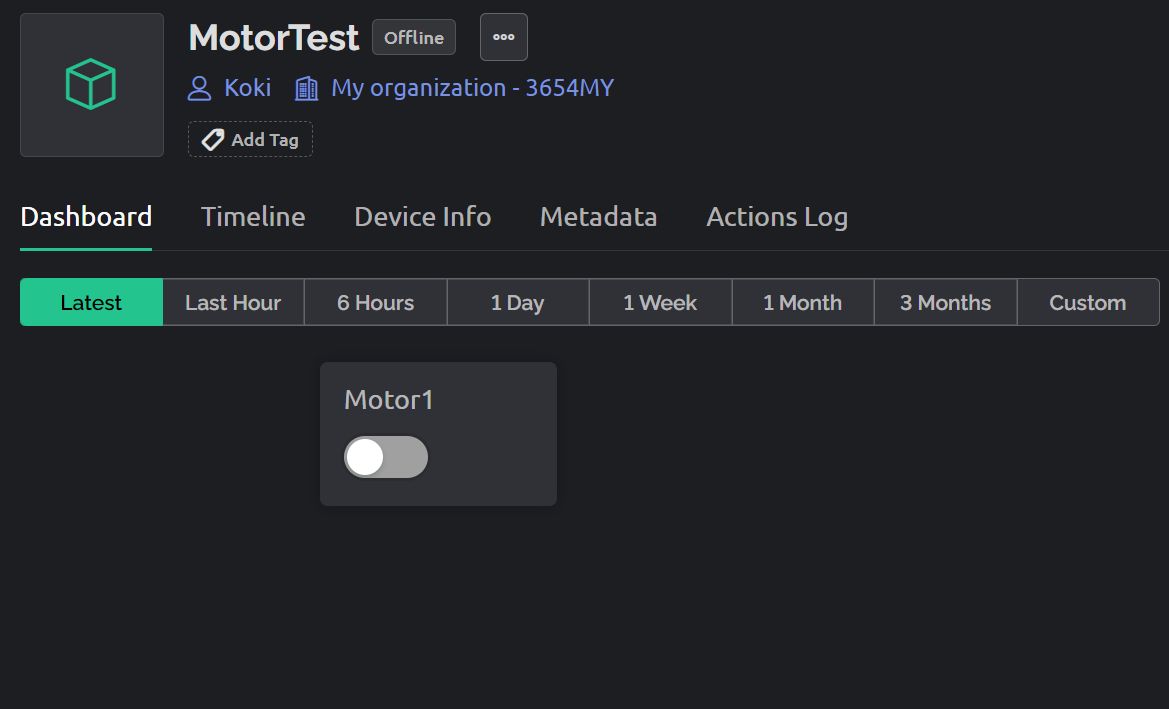
\includegraphics[scale=0.25]
        {figures/BlynkProject.png}
        \caption{Blynkプロジェクト作成画面}
        \label{fig:Blynkプロジェクト作成画面}
      \end{figure}
      
      \begin{figure}[b!]
        \centering
        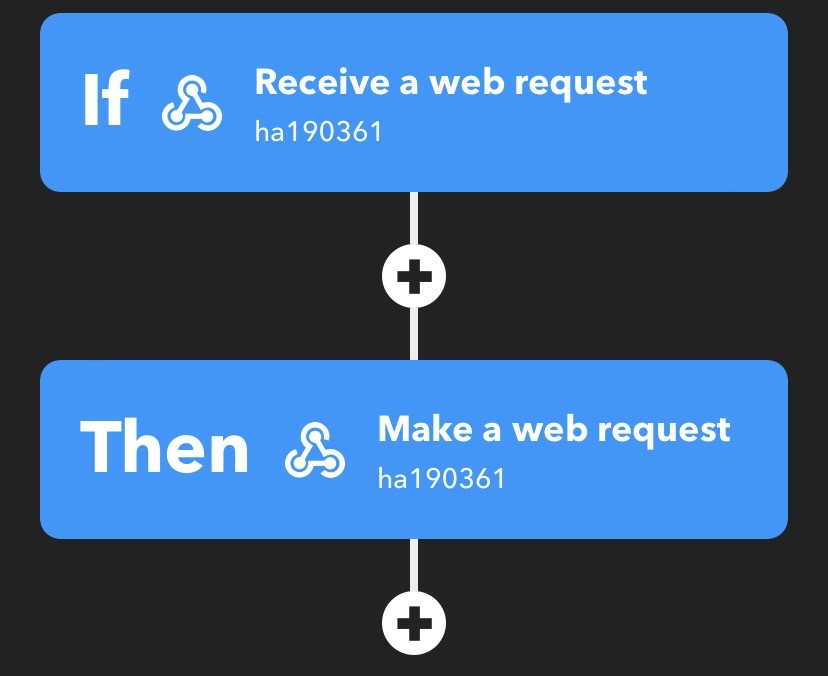
\includegraphics[scale=0.27]
        {figures/IFTTT-overall.jpg}
        \caption{IFTTTを用いて作成したアプレット全体像}
        \label{fig:IFTTTを用いて作成したアプレット全体像}
      \end{figure}
      
      \par 一方で,指紋による認証を用いたソフトウェアの実装については外部アプリケーションを利用せずに指紋認証センサーを用いてネットワークに接続しなくても動作確認ができる状態を構築する.制御方法の概要については図\ref{fig:指紋認証をベースとしたスマートロックの概要図}にて示した通りであるが,ここではより具体的に説明を加える.
      \par NFC認証を利用したスマートロックの実装との差分は指紋認証センサとその配線にあるため,それぞれについて説明する.指紋認証センサーは光学式指紋認証センサーモジュール(ZFM-70シリーズ)を用いて,センサーの5VとGNDの配線についてはマイコンの該当する5Vピンと接地ピンに接続する.センサーの受信用コード(RxD)と送信用コード(TxD)についてはマイコンの任意のピン番号に接続する.なお,本実装についてはそれぞれ19番ピンと18番ピンに接続する.マイコンに書き込むプログラムについては主に指紋の入力・認証処理・モーター回転命令出力の3つに大別される.また,それらとは別に予め指紋登録用のプログラムを書き込むことによって指紋認証センサー上に認証するための指紋情報を登録する.
  
      
      
          
  \subsection{数理最適化モデルの実装}
    \label{sec:数理最適化モデルの実装}
      \par 本節では,\ref{sec:数理最適化ベースのマッチングモデルの設計}節にて定式化した数理最適化モデルを実際のシステムに組み込むための実装手法について説明する.数理最適化モデルの実装においては,効率的かつ正確に解を求めるための適切なソルバーの選定が不可欠である.さらに,選定したソルバーを用いて,アルゴリズムをどのように実装するかも重要な課題である.以下では,まず\ref{sec:ソルバーの選定}項にてソルバーの選定について詳細に議論し,その後,\ref{sec:アルゴリズムの実装}項にてアルゴリズムの具体的な実装方法について述べる.
      
      \subsubsection{ソルバーの選定}
        \label{sec:ソルバーの選定}
          \par ソルバーの性能は,結果の質や計算時間に大きく影響するため,自転車割り当て問題を効率的かつ正確に解くためには適切なソルバーの選定が必要不可欠である.特に,CtoCシェアサイクルシステムにおいては,リアルタイム性やスケーラビリティが求められるため,最適なソルバー選定がシステム全体のパフォーマンスを左右する.
          
          \par 本研究で扱っている自転車割り当て問題の特徴としては,整数線形計画問題として定式化される点が最大の特徴として挙げられる.他にも,変数にはバイナリ値のみが含まれ,制約条件は線形である点も特徴として挙げられる.問題の規模感としては,シェアリングの対象となる自転車の数やユーザーの需要などに応じて決定変数である二値変数行列の成分の数が大規模になる可能性も考えられる.そのような状況下においても最適な自転車をユーザーに割り当てる必要があるため,解の精度は高く保たれる必要がある.さらに,リアルタイム性が求めらる点も考慮すると,迅速な計算処理を継続して行う必要もある.
          
          \par そこで,ソルバーを選定するにあたって,上記の要件を満たすための観点をいくつかまとめる.まず性能面において,大規模問題でも迅速に解を求められ,効率的なメモリ管理が可能であることや,整数線形計画問題に対応していることが求められる.また,利便性の面において,無料で利用可能であることや,アルゴリズムの実装の際に用いるOR-Toolsとの互換性も求められる.なお,OR-ToolsとはGoogle社から提供されている組み合わせ最適化向けのオープンソースソフトウェアであり,非常に広範な可能性のあるソリューションの中から問題に対する最適化ソリューションを見つけ出すことをサポートする\cite{OR-Tools}.
          
          \par 具体的なソルバーの例として,CPLEXやGurobiなどが挙げられる.CPLEXはIBM社から提供されている,混合整数計画法のための分散型並列アルゴリズムと,線形計画,混合整数計画などのための柔軟で高性能な数理計画法ソルバーである\cite{CPLEX}.GurobiはGurobi社から提供されているソルバーであり,並列処理を最大限活用するよう構築され,高度なMIPヒューリスティックアルゴリズムにより実現可能解を素早く求解可能である特徴を持つ\cite{Gurobi}.しかし、これらのソルバーはオープンソースではないが故に,ライセンス費用の面における制限が懸念される.
          
          \par オープンソースソルバーの例としては,GLPKやCBCなどが挙げられる.
          
          \par GLPKはモスクワ航空大学のAndrew Makhorin氏によって開発されたソルバーである.C言語で記述されており,コマンドラインまたはAPIを介して操作可能であり,CとJavaのAPIを提供している.CPLEXのような商用ソルバーと比較するとGLPKの速度は劣るものの,線形計画問題に対して有効なソルバーである\cite{gearhart2013comparison}.
          
          \par CBCはJohn Forrest氏らによって開発された,COIN-OR線形計画法を用いた混合整数計画問題を解くためのソルバーである.C++で書かれており,呼び出し可能なライブラリとしても,スタンドアロンの実行ファイルとしても利用可能である.様々なモデリングシステムやパッケージなどを通して,様々な方法で利用することができる\cite{CBC}.
          
          \par また,オープンソースソルバーの別の例としてSCIPも挙げられる.SCIPは,混合整数線形計画問題や混合整数比線形計画問題,さらには制約整数計画問題のソルバーとして設計された,制約整数計画ソルバーである\cite{bolusani2024scip}.SCIPソルバーは汎用性の高いフレームワークであり,問題のサイズを縮小する前処理や下界値を強化するカット生成,より良い上限値を与えるためのヒューリスティック解法などの機能をプラグインとして追加することができる.これによってSCIPソルバーの利用者は問題に合わせてカスタマイズし,性能を向上させることができる\cite{shinano2013CIPSolver}.一方で,SCIPを利用することの欠点としては,高機能であるが故に複雑性が高く,ある程度の学習コストを要する点や,多数のパラメータを持ち,その設定によって性能が大きく変化するため,最適なパラメータを見つけるためのチューニングが難しい場合がある.
          
          \par 上記で述べた要件やソルバーの一長一短を鑑み,本研究ではSCIPを自転車割り当てにおける整数線形計画問題のソルバーとして選定する.選定理由の最も大きなポイントとしては,オープンソースのソルバーであり,利用するにあたってライセンス関連のコストを懸念する必要が無い点である.オープンソースソルバーとしてSCIP以外に挙げたGLPKやCBCと比較して計算速度が優位である点もSCIPを選定したポイントの1つである.さらに,アルゴリズムの実装の際に用いるOR-Toolsとの互換性が高い点も選定ポイントとして挙げられる.SCIPを利用する際のデメリットとして挙げた複雑性について,OR-Toolsを併用して利用した場合,比較的シンプルにアルゴリズムを実装することが可能となるため,SCIPの長所を最大限生かした実装を行えることが期待される.
          
      \subsubsection{アルゴリズムの実装}
        \label{sec:アルゴリズムの実装}
          \par 本研究で提案する数理最適化ベースの自転車割り当てアルゴリズムは,単にユーザーの最短距離に配置されている自転車を割り当てるわけではない.複数のリクエストをストックした上で,\ref{sec:数理最適化ベースのマッチングモデルの設計}節で定義した目的関数や制約条件のもと,ユーザーの移動後の自転車の配置が全体最適となるように割り当てることによって,CtoCシェアサイクルサービスを実現させることを目的としている.
          \par そこで,実際に\ref{sec:ソルバーの選定}項にて選定したSCIPソルバーを用いて数理最適化ベースの自転車割り当てモデルをモジュールとして実装する.実装する際にはプログラミング言語Pythonを利用する.Pythonとは,1991年にGuido van Rossum氏によって開発されたプログラミング言語であり,コードの可読性を重視した設計哲学や動的型付け言語でありコンパイルが不要である点,包括的な標準ライブラリがサポートされている点などが特徴として挙げられる\cite{aboutPython}.その他,主要なライブラリ及びパッケージとしてSciPyやNumpy,Pandasなどを用い,開発環境としてGoogle Colaboratoryを利用する.
          \par ユーザーリクエストをストックするために定義されるある時間幅に対して処理を実行するアルゴリズム全体のフローチャートは図\ref{fig:自転車割り当てアルゴリズムのフローチャート}で示す通りである.ただし,割り当てモデルクラスをインスタンス化する際のパラメータとして,データフレーム型の地理情報データとシェアリングされる自転車データ$B$を指定する.そうすることによって,指定された地域の特性や利用可能な自転車の数,及びステータスに対して柔軟に対応可能となる.なお,ここで用いる記号で説明を省略している場合は,表\ref{tab:記号の概説}の通りとする.
          \par 距離行列の生成では,入力されるリクエストデータや自転車のステータスから自転車の現在地や自転車の所有者までの位置,ユーザーの現在地などの位置情報を取得し, 測地線距離を用いてそれぞれの対象間の距離を計算し,行列として値を格納する.測地線距離とはリーマン多様体上の2点間の最短経路の長さとして定義\cite{shuvo2024geodesic}され,空間の曲率を考慮した距離を算出する.さらに,距離のスケールを統一するため,生成した距離行列に対してデータの平均が0,標準偏差が1になるよう正規化を実施する.これにより,モデルクラスをインスタンス化する際の地理情報データに依存せず,一貫性を持ったパラメータの調整を行うことができる.
          \par 利用可能な自転車$B_{\text{able}}$は二値行列であり,リクエストされた時刻とシェアリング対象自転車の集合$B$の貸し出し終了日時カラムの値を元に生成される.貸し出し終了日時がNullまたはリクエストされた時刻より過去である自転車は現在利用可能であると判定され1を格納し,それ以外の場合は0を格納する.
          \par データの取得・整形後に数理最適化を実行し,自転車とユーザーの割り当て解が存在するか否かを確認する.解が存在しない場合は処理を終了する.解が存在する場合は,その割り当て解を返し,さらに,シェアリング対象自転車の集合$B$の割り当てられたそれぞれの自転車に対して貸し出し終了日時カラムの値をユーザーリクエストの情報を元に更新する.以降,シェアリング対象自転車の集合$B$を取得する際に,更新された自転車のステータスを元に$B_{\text{able}}$の取得処理が繰り返される.
          \par より大規模なリクエストデータ及び自転車データに対して自転車割り当てアルゴリズムを適用する場合,計算処理に多くのコストを要し,レスポンスまでの待機時間が大幅に上昇する場合がある.レスポンスまでの時間が増大するとユーザー体験は著しく低下し兼ねない.そのため,必要に応じてPythonによるGPU高速計算のためのオープンソースの配列ライブラリCuPyを利用する.CuPyのインターフェースはNumPyと高い互換性を持ち,NumPy配列を定義・利用している箇所をCuPyに置き換えるだけでGPUで並列処理を適切に実行することができ,レスポンスまでの時間を縮小することができる\cite{CuPy}.
          \par エラーハンドリングとして,モデルに入力される値に対しての例外処理を実装する.例えば,インスタンス化する際に入力されるデータフレーム型の地理情報データの経度・緯度カラムに有効な値が格納されているかや,リクエストデータが有効なデータフレームであるかなどの観点が挙げられる.条件分岐による例外出力や随時デバッグ出力にて確認できるよう構築する.

          \begin{figure}[htbp]
            \centering
            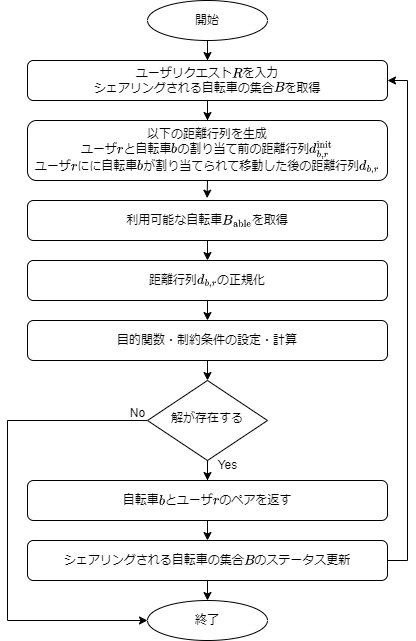
\includegraphics[scale=0.54]
            {figures/algorithmImplementation.png}
            \caption{自転車割り当てアルゴリズムのフローチャート}
            \label{fig:自転車割り当てアルゴリズムのフローチャート}
          \end{figure}
          
  \subsection{API開発}
    \label{sec:API開発}
      \par これまでに実装した自転車割り当てモデルを利用する方法として,本節では,\ref{sec:APIの設計方針}節で策定したAPIの設計に基づき,具体的な実装手順とデプロイメントについて記述する.まず,\ref{sec:APIエンドポイントの実装}節では,スマートロックや自転車割り当てモデルを統合するためのインターフェースとして,APIエンドポイントの実装方法を解説する.ここでは,使用するプログラミング言語やフレームワークの選定理由,および開発環境の構築手順についても言及する.
      \par 次に,\ref{sec:ドキュメンテーションとテスト}節では,APIの品質と信頼性を向上させるためのドキュメンテーションとテスト手法について説明する.APIの利用者やほかの開発者が理解しやすいドキュメントを作成することは,サービスの拡張性や保守性を高める上で重要である.(また,テストの自動化を通じて,将来的な機能追加や変更に対する安定性を確保する方法についても論じる.)
      \par 最後に,\ref{sec:APIデプロイメント}節では,実装したAPIを実際の運用環境にデプロイする手順を紹介する.コンテナ化技術であるDockerを活用したアプリケーションのパッケージング方法や,GCP(Google Cloud Platform)のサービスを利用したデプロイメントプロセスについて詳しく解説する.これにより,開発から運用までの一連の流れを包括的に示し,安定したサービス提供の実現を目指す.
      
      \subsubsection{APIエンドポイントの実装}
        \label{sec:APIエンドポイントの実装}
          \par 実際に\ref{sec:スマートロックプロトタイプ実装}節から\ref{sec:API開発}節までで実装したスマートロックや自転車割り当てモデルを結合するためのインターフェースとして,\ref{sec:APIの設計方針}節にて設計したAPIを実装する.ただし,ここでは軸となる実装部分や利用するツールについての説明に尽力するため,詳細なコードの内容や環境構築手順関しては付録及びREADME.mdを参照されたい.
          \par プログラミング言語はPython,フレームワークはFastAPIを用いて実装する.FastAPIは,文字通りAPI開発に適しており,高速であり,動的型付け言語であるPythonでも型安全な開発を行うことができることが特徴として挙げられる.また,コードを記述することでAPIドキュメントとなるSwagger UIが自動で生成される点も大きな特徴であるが,その点については\ref{sec:ドキュメンテーションとテスト}項にて触れることとする.
          \par APIエンドポイント開発環境として,コードエディタとしてVSCode(Visual Studio Code)を利用することを前提とする.パッケージ管理ツールにはpipenv\cite{pipenv}を用いる.pipenvは,Pythonで書かれた仮想環境及びパッケージ管理ツールである.パッケージの管理を行うツールであるpipと仮想環境を管理するvenvの両方の機能を一つのパッケージ内に兼ね備えており,簡単に開発環境を構築することを可能とする.Pipfile及びPipfile.lockのファイルを元に必要なパッケージを仮想環境にインストールする.
          \par APIサーバーの起動については,ASGI Webサーバー実装のためのツールuvicorn\cite{uvicorn}を利用する.ASGI(Asynchronous Server Gateway Interface)は非同期サーバーゲートウェイインターフェースを意味し,uvicornは軽量で非同期処理可能で効率よくリクエストを処理できるAPIサーバーを立ち上げる際に便利なツールとなる.実際にuvicornはコマンドラインツールとして利用し,コマンドライン引数にFastAPIをインスタンス化しているファイルを指定することでWebサーバーが立ち上がる.
          \par エンドポイントの具体的な実装手順としては,まず,FastAPIをインスタンス化した変数を使用して,任意のリクエストメソッドを処理するデコレータを呼び出して定義する.次に,デコレータ内で呼び出したメソッドの引数にエンドポイントとなるURIを渡す.必要に応じてレスポンススキーマもここで定義し,レスポンスの形式を保証する設定も追加可能である.なお,デコレータとはクラスや関数などの既存オブジェクトに対して,その前後に特定の処理を動的に追加できる機能のことを意味する.既存オブジェクトの先頭にアットマーク(@)で始まる処理が記述されている場合,それはデコレータである.
          \par デコレータにて定義したエンドポイントとリクエストメソッドが実際のリクエストと一致した場合,その直下に定義しているメソッドが発火し,処理が実行され,レスポンスが返ってくる.\ref{sec:API機能要件の定義と設計}項にて定義・設計した全てのエンドポイントに対してデコレータとメソッドを記述することでエンドポイントの準備は完了することになる.可読性の観点から,FastAPIをインスタンス化するファイルとエンドポイントを定義するファイルは別ファイルとして管理する.さらに,エンドポイントを定義するファイルにおいても,マイクロサービスのサービス別にファイルを分離して管理する.
          \par ここで課題となるのが,GETメソッドにてデータを取得したり,POSTメソッドにてデータを保存したりする際のデータの管理や永続化である.そこで,軽量なデータベースエンジンであるSQLite\cite{sqlite}を利用する.また,それに伴い,ORM(Object Relational mapper)としてSQLAlchemy\cite{sqlalchemy}を利用する.これはデータベースのテーブルをオブジェクトとしてマッピングでき,テーブル間のリレーションを簡単に管理することのできるフレームワークである.データベースのテーブルと行のオブジェクトラッパーであるデータマッパーパターンが実装され,SQL文を書く必要が無く,クラスの属性を介してデータフィールドにアクセスすることができる.
          \par APIエンドポイントの追加や改修を行うと,データベースモデルは次第に変化する可能性が大いに考えられる.そこで,SQLAlchemyとシームレスに統合可能なマイグレーションツールAlembic\cite{alembic}を用いる.適宜セットアップや初期化を行い,以後のデータベースの更新に関してはmigrationsディレクトリ内にストックするマイグレーションファイルを元に行う.これによって,データベースを過去の状態に戻すためのロールバックも簡単に実行することができるため,更新後にデータベース周りに不具合が発生した場合,直前の状態に戻すことも選択肢として考えることができる.
          
      \subsubsection{ドキュメンテーションとテスト}
        \label{sec:ドキュメンテーションとテスト}
          \par APIのドキュメンテーションを用意することは開発者同士のコミュニケーションにおいても,API利用者にとっても重要な意義を持つ.APIはある二点間のインターフェースとなり,それぞれのリクエスト形式及びレスポンス形式を定義し,APIを実装する際の軸となるからである.本研究で実装するAPIは,どの地域でもCtoCシェアリングサービスを提供できる拡張性に重きを置いていることから,ドキュメントの対象は,各地域でAPIを実装する外部開発者を想定する.外部開発者が,本研究で構築したAPIを簡単に実装できるようドキュメント化することを最大の目的として据えている.
          \par ドキュメントの生成については,APIのソースコードから自動で定義書を生成するツール「Swagger UI\cite{swagger-ui}」を用いる.Swagger UIはOpenAPIと連携しており,OAS(OpenAPI Specification)形式で記述されたAPI定義書の内容も反映しドキュメントを生成する.さらに,Web UI上にてリクエストパラメータ等を自由に設定しながらデバッグすることも可能である.これらの特徴からドキュメンテーションにSwagger UIを用いることとした.
          \par ドキュメントの作成手順としては,まず,JSON Schemaを用いてリクエストやレスポンス及びそれらのプロパティとなるデータをモデル化する.なお,JSON SchemaとはJSONドキュメントのデータ構造やフォーマットを定義するための仕様である.
          \par 続いて定義したJSON SchemaをJSONポインタを用いてそれぞれのオブジェクト内で呼び出す.なお,JSONポインタとは同一仕様内の別の定義を参照することのできるJSON Schemaの特別な構文である.これを用いることでスキーマの関係を入れ子構造で定義でき,スキーマ定義の繰り返しを避け,可読性やメンテナンス性を向上させることができる.
          \par その後,URLのパスを宣言し,APIのエンドポイントを文書化する.その際,それぞれの宣言したパスの配下にて,クエリパラメータやリクエストペイロード,レスポンスなどの形式を,必要に応じてJSONポインタを指定して定義する.また,それぞれのパスに対してタグの項目を指定し,マイクロサービスごとに分割できるようにする.例を挙げると,自転車管理サービスはBikeタグで,自転車割り当てサービスはDispatchタグで紐づける.
          \par 最後に,APIの認証スキームを定義する.認証が必要なエンドポイント及びメソッドに対して,それぞれのオペレーションIDを明示することで認証を実装することが可能となる.ドキュメンテーションの詳細な実装内容は付録ソースコードのoas.yaml及びREADME.mdを参照されたい.
          \par さらに,テストを用意することにも重要な意義を持つ.テストは既存のコードに対しての信頼性や品質を保証するだけでなく,今後の変更に対する保守性が向上することにも繋がる.そこで,APIがOASに沿った正しい振る舞いをしているかどうかをテスト及び検証するためのライブラリ「schemathesis\cite{schemathesis}」を用いて自動テストを実装する.
          \par schemathesisは,ドキュメント化した定義書を元に,全てのAPIエンドポイントに対して考え得る全てのリクエストパターンをテストケースとして自動生成する.定義書にAPI間のリレーションも明記すれば,そのリレーションも考慮したテストケースも追加で生成することが可能である.本記事執筆時点で実装されている5つのエンドポイントに対して900以上ものテストケースが自動で生成される.必要に応じてテストで落ちている箇所を修正することで堅牢なAPIを実装することができる.
          \par 今回は採用しなかったが,別のAPIテスト戦略として,APIテストフレームワークであるDreddやプロパティベースのテストを実行することができるPythonライブラリのHypothesisなどを用いたテストを設計することも可能である.
          \par Dreddを用いる場合の特徴としては,フックと呼ばれる概念にある.各エンドポイントのテストの実行前後に,beforeフックまたはafterフックを用いてテストのサンプルとなる状態をカスタマイズする.しかし,Dreddは正常系のテストは実装可能である一方,異常系のテストには不十分であり,また,カスタマイズに時間的リソースが割かれることから本研究では採用していない.
          \par Hypothesisを用いる場合の特徴としては,メソッドの戻り値のプロパティに対してアサーションを作成する点にある.正常系のメソッドの他,異常系のメソッドに対応しており,スキーマで定義されたデータに対して,スキーマが期待するデータ型以外のパラメータも自動で生成し,検証することができる.ただ,Schemathesisのリンク機能が無いなど,Schemathesisの下位互換的立ち位置であるため,本研究では採用していない.
      
      \subsubsection{APIデプロイメント}
        \label{sec:APIデプロイメント}
          % \par $\Box$ CI/CDパイプラインへの統合
          \par APIをデプロイするにあたり,前述した\ref{sec:APIエンドポイントの実装}項及び\ref{sec:ドキュメンテーションとテスト}項より,ローカル環境におけるAPIの実装が完了済みでテストもパスしている状態であることを前提とする.また,デプロイには外部サービスを利用してる側面もあり,別途費用が発生する点にご留意いただきたい.
          \par まずはAPIアプリケーションをDocker化する必要がある.Docker化とは,アプリケーションをDockerイメージとしてパッケージ化する工程のことを意味し,ここでは,マイクロサービスとして定義した自転車管理サービスと自転車割り当てサービスを統合した形でDockerイメージを作成する.これにより,アプリケーションを環境から独立させ,可搬性や再現性が向上し,様々な環境でアプリケーションをデプロイすることが可能となる.
          \par DockerイメージをビルドするためにDockerfileを作成する必要がある.ベースイメージとして,公式のPyton 3.10のDockerイメージの軽量バージョンを利用する.利用するために,DockerのFROMディレクティブを用いて該当のベースイメージを利用することを指定する.続いてDockerのRUNディレクティブを用いて,アプリケーションコード用の作業ディレクトリを作成する.その後,DockerのWORKDIRディレクティブを用いて作成したディレクトリを作業ディレクトリとして設定する.アプリケーションは設定された作業ディレクトリにて実行される.
          \par 次にDockerのRUNディレクティブを用いて,pip及び依存関係ツールのpipenvをインストールする.DockerのCOPYディレクティブを用いて,アプリケーションの依存関係を記述したPipfileとPipfile.lockをコンテナ内の作業ディレクトリにコピーする.その後,pipenvを使用して,システム環境に必要なパッケージをインストールする.ここで,--deployオプションをコマンドに含めることによってPipfile.lockと一致しない変更が存在する場合にはエラーを出力し,Pipenvが常に最新であることを保証する.この際,アプリケーションはDockerで実行されるため,Docker導入以前に利用していた仮想環境は必要なくなることに注意する.
          \par 最後に,プロジェクト全体のアプリケーションコードをコンテナ内の作業ディレクトリにコピーする.コンテナがリッスンするポートをDockerのEXPOSEディレクティブを用いて指定し,アプリケーションを稼働させるために必要な実行コマンドをDockerのCMDディレクティブを用いて指定する.
          \par Dockerイメージがビルドされる際はDockerfileの各ステップが上から順にキャッシュされるため,記述順序が非常に重要となる.実際の構築に用いたDockerfileは付録を参照されたい.
          \par ビルドしたDockerイメージを利用するため,GCR(Google Container Registry)へDockerビルドを公開する.GCRとはGoogle社より提供されているGCP(Google Cloud Platform)のサービスの1つで,プライベートなDockerイメージのレジストリサービスである.
          \par その後,ビルドしたDockerイメージを用いて,Cloud Runにサービスをデプロイする.Cloud RunもGCRと同様にGCPのサービスの1つであり,サーバーレスのフルマネージドコンテナ実行環境を提供している.コマンドからCloud Runへサービスをデプロイする際に4つのオプションを設定する.--imageオプションで使用するDockerイメージ指定し,--platformオプションでマネージドプラットフォームを指定する.さらに--regionオプションで東京のリージョン名を指定し,--allow-unauthenticatedオプションで認証無しによるアクセスを許可する.
          \par 環境変数を設定する必要がある場合は別GCPのコンソール画面から操作する.該当するCloud Runサービスの編集画面から環境変数セクションにアクセスすることができるため,そこで設定が可能である.本アプリケーションの場合,データベースのURLを環境変数に格納した上でソースコードで扱っている.
          \par デプロイが成功したら,サービスのURLにアクセスして動作を確認する.APIデプロイメント成功後の全体像は図\ref{fig:APIデプロイ後のクラウドアーキテクチャ}のようになる.Dockerにてコンテナ化している部分で,Next.jsの表記が確認できる.これはAPIドキュメントをホスティングするにあたってフロントエンドとしてページを表示させるために用いたものである.また,必要不可欠ではないが,適宜ドメイン名を紐付けてURLをカスタムドメイン化する選択肢もある.

          \begin{figure}[htbp]
            \centering
            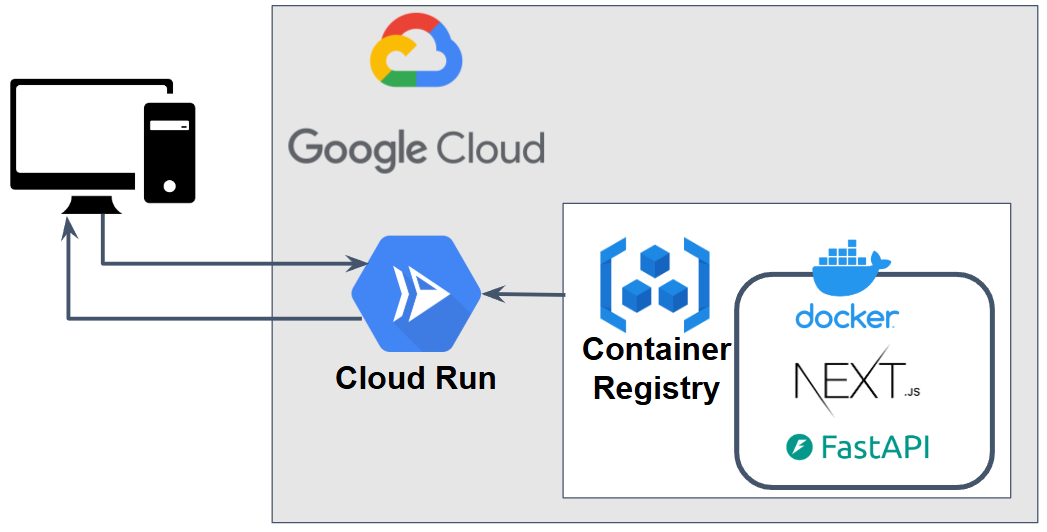
\includegraphics[scale=0.28]
            {figures/TechStack.png}
            \caption{APIデプロイ後のクラウドアーキテクチャ}
            \label{fig:APIデプロイ後のクラウドアーキテクチャ}
          \end{figure}
